\subsection{Distributed approach}
\label{subsec:ex1distr}

\subsubsection{Model training}
\label{subsubsec:learneddist}

Once, enough data are collected through the simulator by using the optimal 
controller, it is possible to train a very simplified ``distributed network'' 
that takes as input an array containing the response values of the sensors – 
which can be either \texttt{prox\_values}, \texttt{prox\_comm} or 
\texttt{all\_sensors} – and produces as output an array containing one float 
that represents the speed of the wheels, which is assumed to be the same 
both right and left.

The dataset then contains a fixed number of simulation runs, each of these 
composed by a variable quantity of timesteps. It is important to notice that 
for this approach, unlike the one with communication, it is not necessary to 
keep the order of the sequence of timesteps, neither to know the exact 
number of agents in the simulation since the network input is the sensing 
associated to a single robot.

For this reason, the model is independent of the number of agents and 
consequently it is possible to prove its generalisation capacity, regardless 
the number of robots, by training the networks first on datasets each with a 
different but fixed value of $N$ and then on simulations composed by a 
variable $N$.
It is easy to show that although the value of $N$ changes the network 
structure does not, as it is sufficient during the input preprocessing to 
change the dimension of the input in such a way that all the tensors have a 
the same length, fixed at the maximum possible value of $N$, padding 
those tensors with a lower number of agents.

Thanks to these two assumptions, it is possible to shuffle the original 
dataset, based on the single run, in order to improve the generalisation on 
the samples, and then split the resulting collection into the train, the 
validation and the test sets, containing respectively $60$-$20$-$20\%$ of 
the data. 

The architecture of the network, displayed in Figure 
\ref{fig:singlenetdistributed1}, is straightforward: there are three linear 
layers each of size $\langle\mathtt{input\_size}, 10\rangle$,  $\langle 10, 
10\rangle$ and $\langle 10, 1\rangle$, where \texttt{input\_size} is the 
shape of the sensing, that can be $7$ or $14$.
\begin{figure}[htb]
	\centering
	\begin{subfigure}[h]{0.495\textwidth}
		\centering
		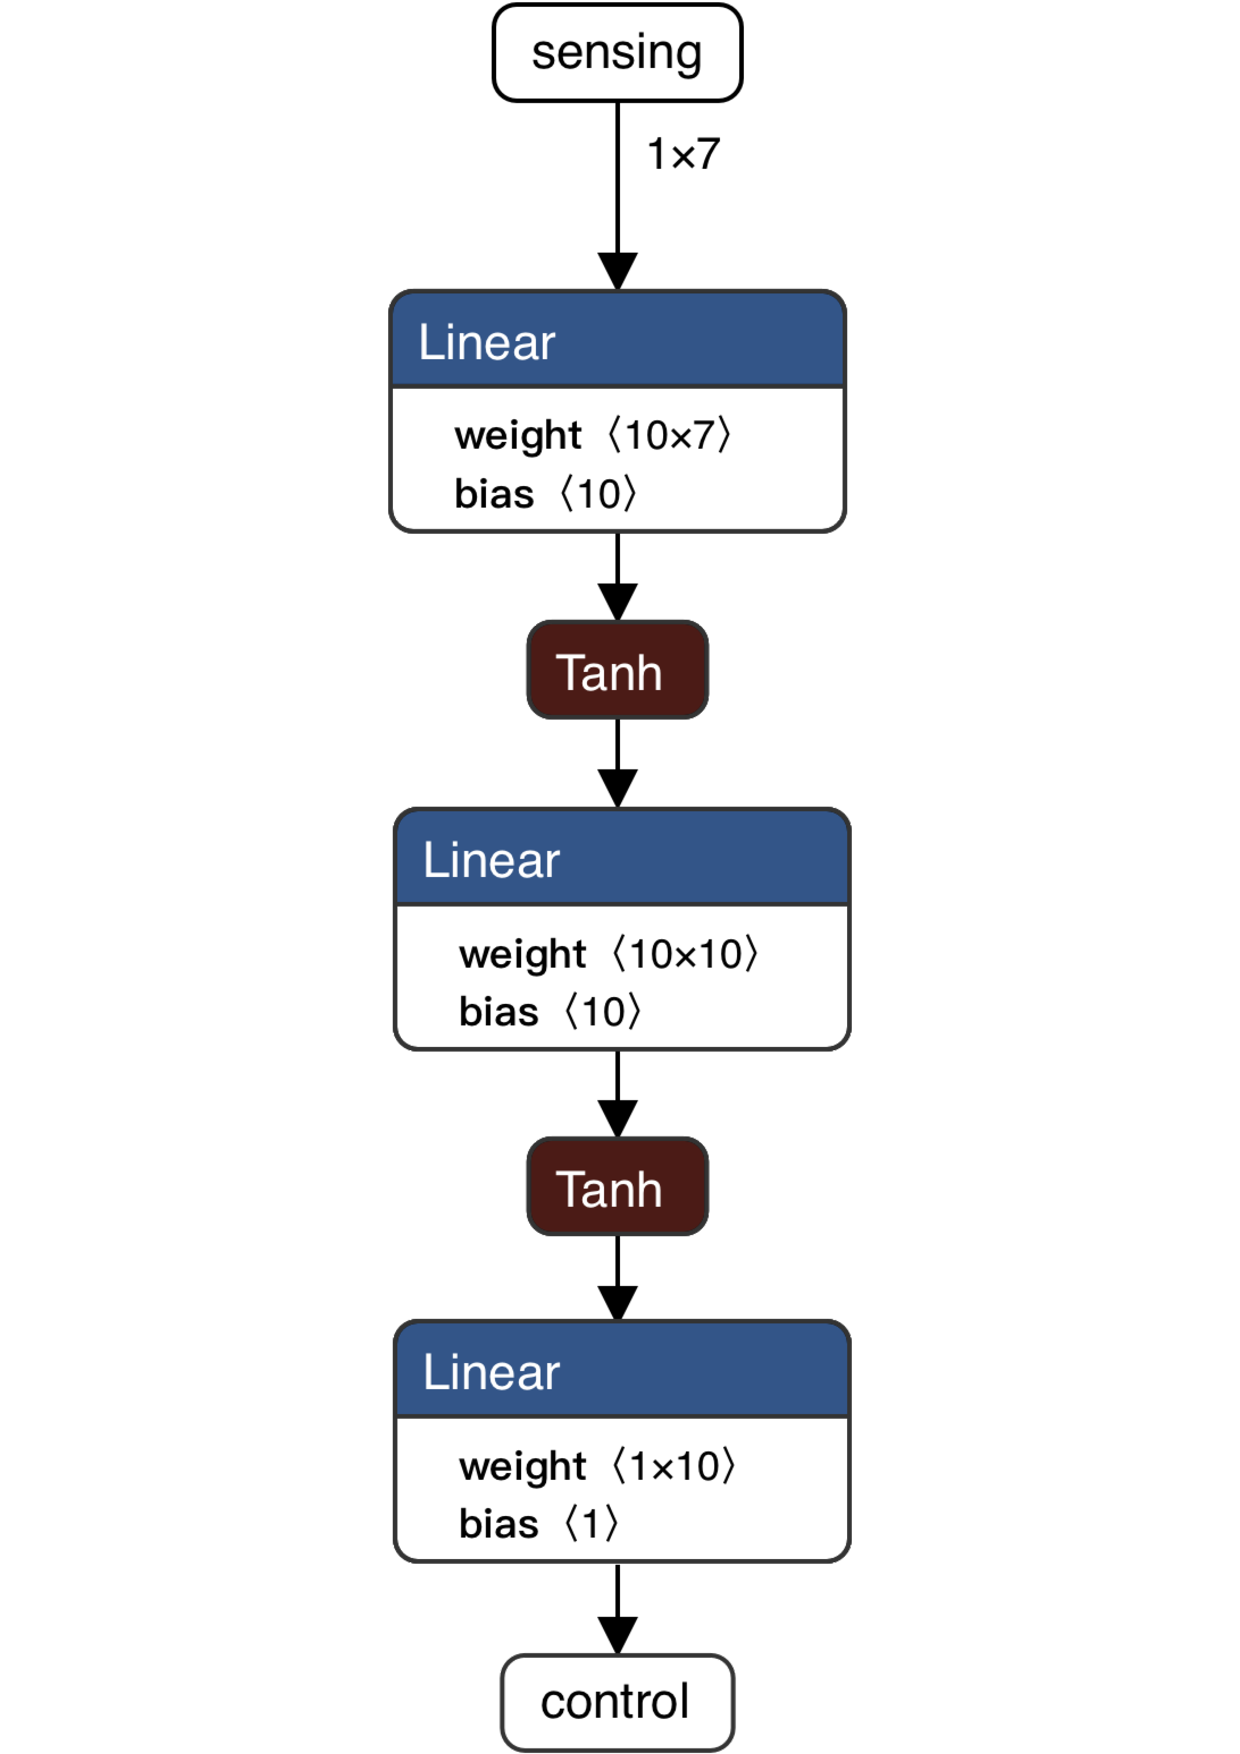
\includegraphics[width=.3\textwidth]{contents/images/task1distributed@4x}%
		\caption{Network with $7$ input sensing.}
		\label{fig:singlenet7distributed1}
	\end{subfigure}
	\hfill
	\begin{subfigure}[h]{0.495\textwidth}
		\centering
		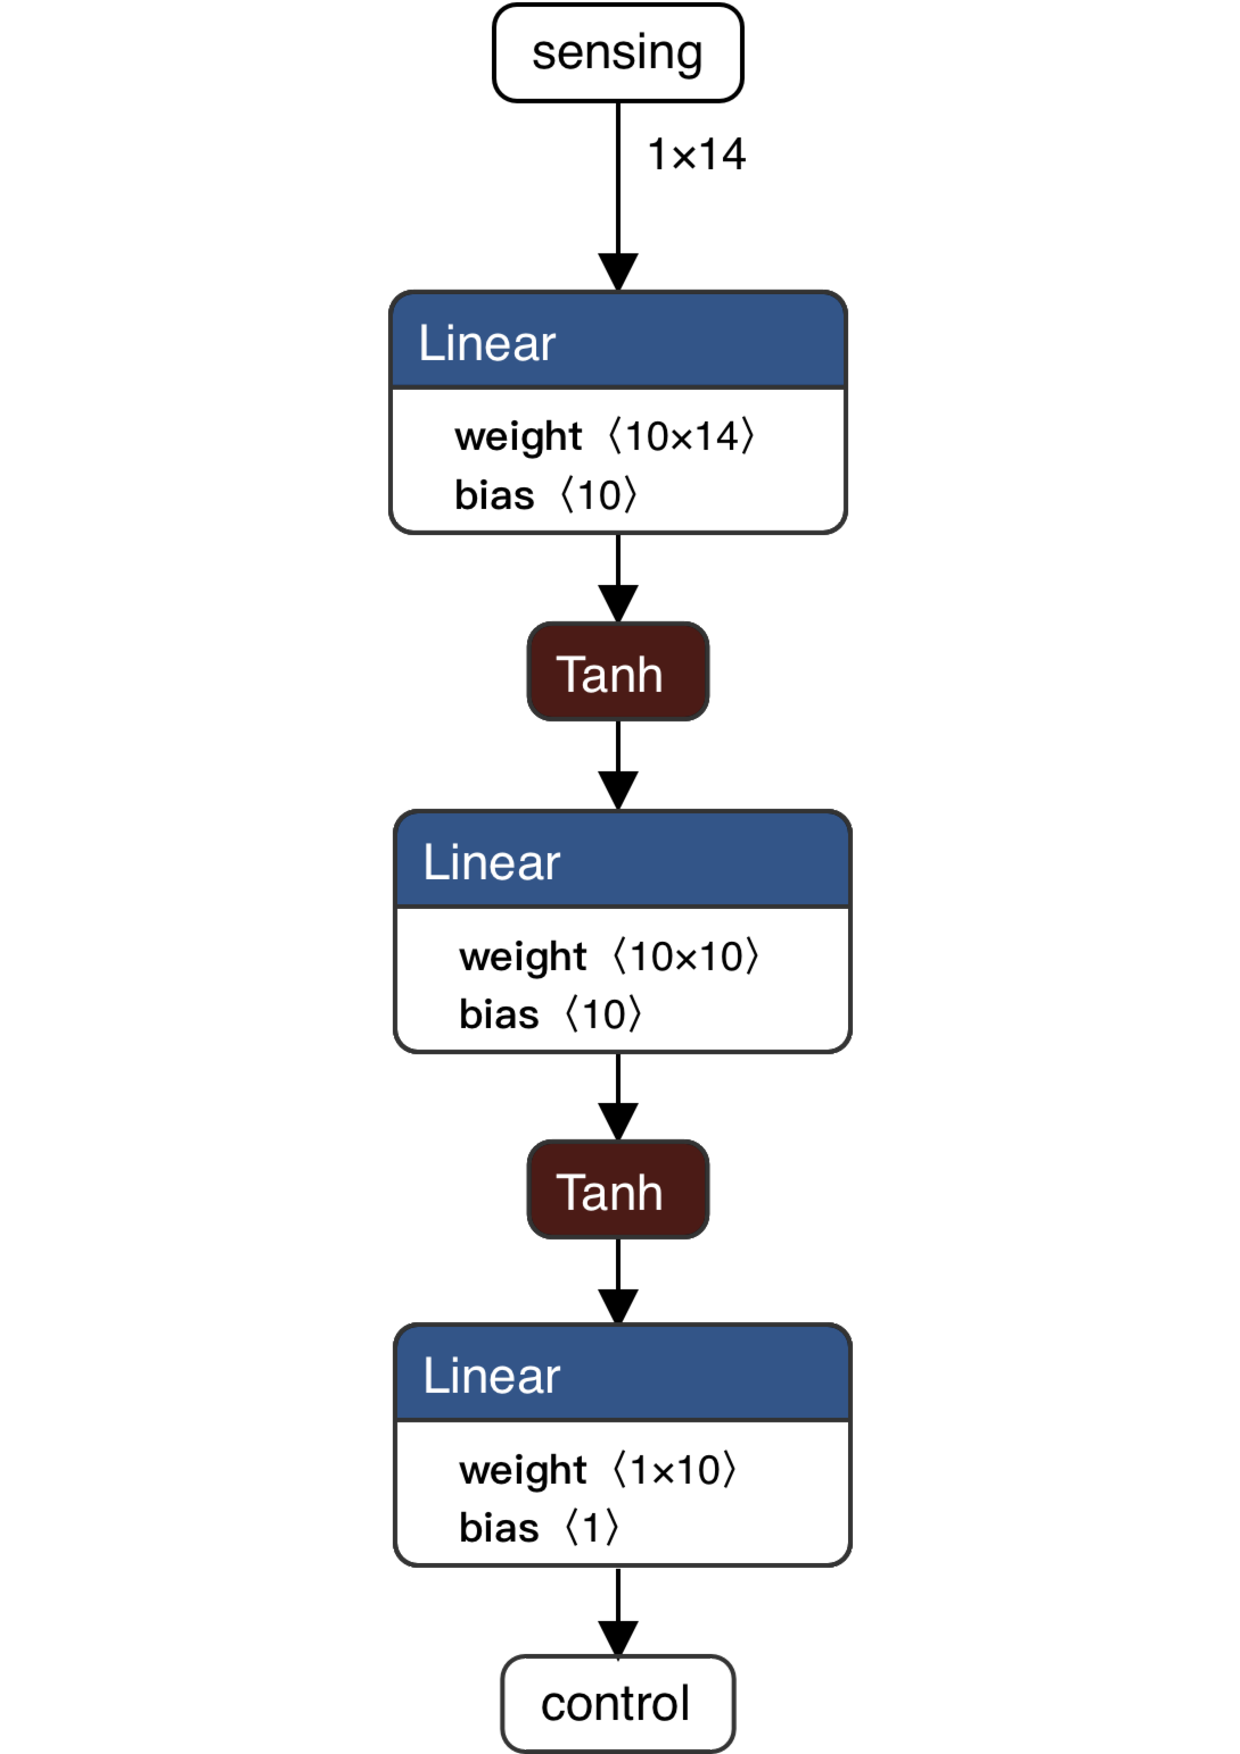
\includegraphics[width=.3\textwidth]{contents/images/task1distributed_all@4x}
		\caption{Network with $14$ input sensing.}
		\label{fig:singlenet14distributed1}
	\end{subfigure}
	\caption[Network architectures for the distributed approach.]{Visualisation of 
	the network architectures for the distributed approach.}
	\label{fig:singlenetdistributed1}
\end{figure}
To the first and second layer is applied a non-linear activation function, 
useful to make the model generalise. 
In particular, we chose the hyperbolic tangent (Tanh) 
\cite[see][]{kalman1992tanh}, a zero-centred function, shown in Figure 
\ref{fig:tanh}, whose range lies between $[-1, 1]$ and its output is given by

\begin{Equation}[H]
	\centering
	\begin{equation}
	f(x)= \frac{\sinh (x)}{\cosh (x)} = \bigg( \frac{e^x - e^{-x}}{e^x + 
		e^{-x}}\bigg)
	\end{equation}
	\caption{Hyperbolic Tangent Function (Tanh).}
	\label{eq:tanh}
\end{Equation}

This type of activation function is often used in deep learning and one of is 
advantages is that negative inputs are mapped to strongly negative values.

\begin{figure}[!htb]
	\centering
	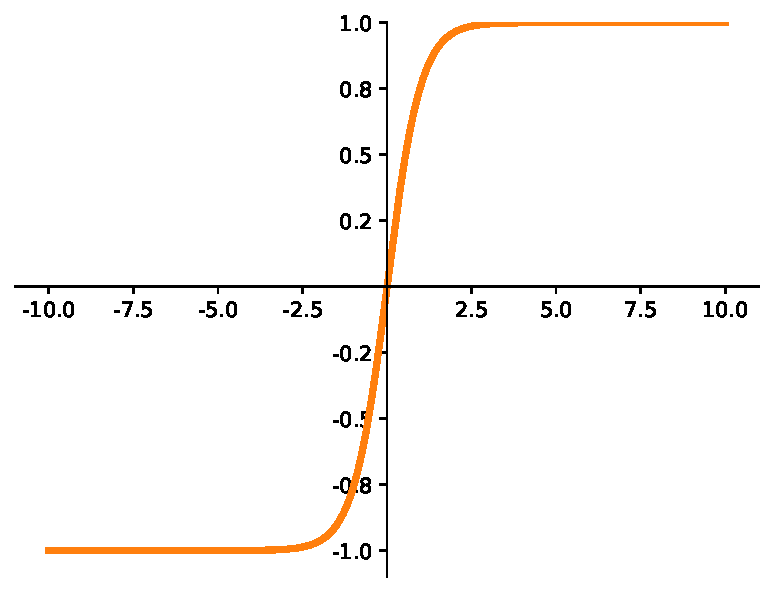
\includegraphics[width=.5\textwidth]{contents/images/tanh2}%
	\caption{Trend of the Tanh activation function.}
	\label{fig:tanh}
\end{figure}

%fixme citation
As optimiser we chose Adam, {an algorithm for first-order gradient-based 
optimisation of stochastic objective functions, based on adaptive estimates of 
lower-order moments}, \cite[see][]{kingma2014adam, 
loshchilov2017decoupled}, 
implemented in the \texttt{torch.optim} package, with a learning rate of $0.01$. 

Instead of computing the gradient descent on the entire dataset, the training set is 
split in mini-batches of size $100$ and an approximation of the gradient is 
produced, which makes the algorithm faster and at the same time, for sufficiently 
large numbers, the result is indistinguishable.

Gradient descent algorithms are susceptible to ``get stuck'' in local minima.
Mini-batches shuffle facilitate to avoid this problem by enabling the gradient to 
``bounce'' out of eventual local minimum, making it more variable by exploiting 
randomness, thereby helping convergence.

All the models are trained for $50$ epochs and evaluated using the \gls{mse} loss 
function, often used in regression problems. 
This criterion, implemented in the \texttt{torch.nn} package, measures the 
average of squared error between predictions and targets and learns to reduce it 
by penalising big errors in the model predictions.

\begin{Equation}[!htb]
	\centering
	\begin{equation}
	\mathtt{MSE} = \frac{\sum_{i=1}^n (y_i-\hat y_i)^2}{n}
	\end{equation}
	\caption{Mean Squared Error (\gls{mse}) loss function.}
	\label{eq:mse}
\end{Equation}
	

\subsubsection{Experiments}
\label{subsubsec:expdist}

The first group of experiments carried out, summarised in Table 
\ref{tab:modeln5dist}, examines the behaviour of the control learned in the case 
of the three different inputs, \texttt{prox\_values}, \texttt{prox\_comm} or 
\texttt{all\_sensors}, for a number of robots $N$ and an \texttt{avg\_gap} both 
fixed respectively at $5$ and the second chosen between $8$, $13$ and $24$.
\begin{figure}[H]
	\centering
	\begin{tabular}{llrr}
		\toprule
		\textbf{Model} \quad & \textbf{\texttt{network\_input}} & 
		\textbf{\texttt{input\_size}} &
		\textbf{\texttt{avg\_gap}} \\
		\midrule
		\texttt{net1} 				 & \texttt{prox\_values}	&  $  7$  &  $  8$  \\
		\texttt{net1b} 				& \texttt{prox\_values}	   &  $  7$  &  $13$ \\
		\texttt{net1c} 				& \texttt{prox\_values}	   &  $  7$  &  $24$  \\
		\texttt{net2} 				 & \texttt{prox\_comm}	  &  $  7$  &  $  8$  \\
		\texttt{net3} 				 & \texttt{prox\_comm}	  &  $  7$  &  $13$  \\
		\texttt{net4} 				 & \texttt{prox\_comm}	  &  $  7$  &  $24$  \\
		\texttt{net5} 				 & \texttt{all\_sensors}	  &  $14$  &  $  8$  \\
		\texttt{net6} 				 & \texttt{all\_sensors}	  &  $14$  &  $13$ 	\\
		\texttt{net7} 				 & \texttt{all\_sensors}	  &  $14$  &  $24$ 	\\
		\bottomrule
	\end{tabular}
	\captionof{table}{List of the experiments carried out with $5$ agents.}
	\label{tab:modeln5dist}
\end{figure}

First of all we start by showing in Figure \ref{fig:distloss} an overview of the 
models performance in terms of train and validation losses. 
\begin{figure}[!htb]
	\centering
	\includegraphics[width=.8\textwidth]{contents/images/task1/loss-distributed-all@x10}%
	\caption{Comparison of the losses of the models carried out with $5$ agents.}
	\label{fig:distloss}
\end{figure}
It is immediately evident that, in case of \texttt{prox\_values} inputs, the 
experiment performed with an \texttt{avg\_gap} of $24$ is not remarkable since 
this value exceeds the maximal range of the sensor.

We start the analysis by exploring the results of the experiment obtained 
using the \texttt{prox\_values} readings alone as input of the network, continuing 
the with \texttt{prox\_comm} and concluding with \texttt{all\_sensors}.
The performance of \texttt{net1} are shown in the following images. In particular,  
in Figure \ref{fig:net1r2} is visualised a comparison of the \gls{r2}, or coefficient 
of determination, of the manual and the learned controllers, on the validation set.
This score function evidences how well the regression predictions approximate 
the real data points (groundtruth). Since a model that perfectly predicts the data 
has a score of $1$, we assume that a higher score corresponds to a model that 
performs better.
\begin{figure}[!htb]
	\centering
	\begin{subfigure}[h]{0.49\textwidth}
		\centering
		\includegraphics[width=\textwidth]{contents/images/distr-net1/regression-manualvsomniscient}%
		%\caption{Expert controller output velocity.}
	\end{subfigure}
	\hfill
	\begin{subfigure}[h]{0.49\textwidth}
		\centering
		\includegraphics[width=\textwidth]{contents/images/distr-net1/regression-net1-vs-omniscient}
		%\caption{Distributed controller output velocity.}
	\end{subfigure}

	\caption[Evaluation of the \gls{r2} coefficient of \texttt{net1} .]{Comparison of 
	the \gls{r2} coefficient of the manual and the controller learned from 
	\texttt{net1} with respect to the omniscient one.}
	\label{fig:net1r2}
\end{figure}

From these figures we expect that the robots' behaviour using the learned 
controller instead of the manual one is a bit better, even if far from the 
omniscient 
controller.

In Figure \ref{fig:net1traj} we show first a comparison of the expert and the 
learned trajectories, and then between the manual and the learned ones. In 
particular, on the y-axis is visualised the position of each agent over time, while 
on the x-axis the simulation timesteps. It is important to notice that the plots 
summarise all the runs: at each timestep, the position of each agent is presented 
as an average over all the simulation runs, and in addition is  shown this average 
minus and plus the standard deviation.
\begin{figure}[!htb]
	\centering
	\begin{subfigure}[h]{0.49\textwidth}
		\centering
		\includegraphics[width=\textwidth]{contents/images/distr-net1/position-overtime-omniscient}%
		\caption{Expert controller trajectories.}
	\end{subfigure}
	\hfill
	\begin{subfigure}[h]{0.49\textwidth}
		\centering
		\includegraphics[width=\textwidth]{contents/images/distr-net1/position-overtime-distributed}
		\caption{Distributed controller trajectories.}
	\end{subfigure}
	\hspace*{\fill}%          % empty line absolutely necessary!
	
	\vspace*{8pt}%  
	
	\hspace*{\fill}%  
	\begin{subfigure}[h]{0.49\textwidth}
		\centering
		\includegraphics[width=\textwidth]{contents/images/distr-net1/position-overtime-manual}%
		\caption{Manual controller trajectories.}
	\end{subfigure}
	\hfill
	\begin{subfigure}[h]{0.49\textwidth}
		\centering
		\includegraphics[width=\textwidth]{contents/images/distr-net1/position-overtime-distributed}
		\caption{Distributed controller trajectories.}
	\end{subfigure}
	\caption[Evaluation of the trajectories learned by \texttt{net1}.]{Comparison 
		of trajectories generated using three controllers: the expert, the manual and 
		the one learned from \texttt{net1}.}
	\label{fig:net1traj}
\end{figure}

The convergence of the robots to the target using the omniscient controller is 
much faster than that with the manual or the learned one. In particular, the 
learned trajectories, even if converge to the correct configuration they require a 
higher number of timesteps, sometimes even 40 timesteps may be necessary, 
compared to the two others controllers, where less than 10 timesteps are 
sufficient.

\begin{figure}[!htb]
	\centering
	\begin{subfigure}[h]{0.3\textwidth}
		\centering
		\includegraphics[width=\textwidth]{contents/images/distr-net1/control-overtime-omniscient}%
		\caption{Expert controller.}
	\end{subfigure}
	\hfill
	\begin{subfigure}[h]{0.3\textwidth}
		\centering
		\includegraphics[width=\textwidth]{contents/images/distr-net1/control-overtime-manual}%
		\caption{Manual controller.}
	\end{subfigure}
	\hfill
	\begin{subfigure}[h]{0.3\textwidth}
		\centering
		\includegraphics[width=\textwidth]{contents/images/distr-net1/control-overtime-distributed}
		\caption{Distributed controller.}
	\end{subfigure}
	\caption[Evaluation of the control learned by \texttt{net1}.]{Comparison 
		of output control generated using three controllers: the expert, the manual 
		and the one learned from \texttt{net1}.}
	\label{fig:net1control}
\end{figure}

In fact, analysing in Figure \ref{fig:net1control} the evolution of the control over 
time, it is possible to notice that the omniscient in the first timesteps uses a 
higher speed than that chosen by the manual controller or the one predicted by 
the network. After about $10$ timesteps they both reach the target, with a 
certain tolerance, maintaining then the speed constant at $0$. Instead, the 
distributed controller decreases the speed of the agents as the timesteps pass, 
reaching zero speed but with a certain variance.

A couple of useful plots are shown below. In Figure \ref{fig:net1responsesensors} 
is visualised the response of the learned controller as the input sensing changes. 
\begin{figure}[!htb]
	\centering
	\begin{subfigure}[h]{0.49\textwidth}
		\centering
		\includegraphics[width=\textwidth]{contents/images/distr-net1/response-net1-front}%
		%\caption{response-net1-net([0, 0, x, 0, 0, 0, 0]).}
	\end{subfigure}
	\hfill
	\begin{subfigure}[h]{0.49\textwidth}
		\centering
		\includegraphics[width=\textwidth]{contents/images/distr-net1/response-net1-rear}
		%\caption{response-net1-net([0, 0, 0, 0, 0, x, x]).}
	\end{subfigure}
	\caption[Response of \texttt{net1} by varying the input sensing.]{Response of 
		\texttt{net1} by varying the input sensing.}
	\label{fig:net1responsesensors}
\end{figure}

In particular we analyse two cases. The first one shows the control predicted by 
the network when the robot sees nothing behind but only in front, more 
specifically when the given input is  $([0, 0, x, 0, 0, 0, 0])$, with $x$ varying in the 
range $[0, 4500]$.
The second shows the control predicted by the network when the robot instead 
sees nothing in front but only behind, more specifically when the given input is  
$([0, 0, 0, 0, 0,x , x])$, with $x$ varying in the range $[0, 4500]$.

The behaviour is almost as expected. When the robot sees nothing behind but 
something in front, the model returns a negative speed, since the robot has to 
move backwards. 
The absolute value of control increases as the proximity to the obstacle increases.
The same behaviour is obtained when the robot sees only behind but nothing in 
front. In this case the speed has the opposite sign.

In Figure \ref{fig:net1responseposition} another informative plot displays the 
behaviour of a robot located between two that are already in their place.
It visualises the response of the learned controller by varying the distance 
between two stationary agents and a robot located halfway between them.
On the x-axis is visualised the position of the moving robot, while on the y-axis 
the output control, computed as an average over $100$ measures in which the 
pose of the agent $(x, y, \theta)$ differs by a certain epsilon uniformly distributed 
in the range $[-0.5, 0.5]$. In this way, the result obtained avoids the effects of 
noise that would be obtained on a single measurement and unrealistic artefacts in 
which the sensors are not continuous, compared to the pose, in simulation. In 
addition are also shown the bands that represent plus and minus standard 
deviation.
\begin{figure}[!htb]
	\centering
	\includegraphics[width=.5\textwidth]{contents/images/distr-net1/response-varying_init_position-net1}%
	\caption{Response of \texttt{net1} by varying the initial position.}
	\label{fig:net1responseposition}
\end{figure}

As expected, the output is a high positive value when the robot is close to an 
obstacle on the left, it decreases and reaches $0$ when the distance from right 
and left is equal, and finally becomes negative when there is an obstacle in front 
and not behind.

Finally, in Figure \ref{fig:net1distance} is presented another useful metric that 
measures the absolute distance of each robot from the target, visualised on the 
y-axis, over time. This value is averaged on all robots among all the simulation 
runs. The median value is shown as well as the interquartile and interdecile ranges.
\begin{figure}[!htb]
	\centering
	\includegraphics[width=.7\textwidth]{contents/images/distr-net1/distances-from-goal-compressed-distributed}%
	\caption[Evaluation of \texttt{net1} distances from goal.]{Comparison of 
	performance in terms of distances from goal obtained using three controllers: 
	the expert, the manual and the one learned from \texttt{net1}.}
	\label{fig:net1distance}
\end{figure}
On average, the distance from goal of the learned controller is lower than the one 
obtained with the manual controller, that means that in the final configuration 
the robots moved following the learned controller are closer to the target than 
those moved with the manual one, which are on average at a distance of about 
$1$ \gls{cm} from the goal position. 

As mentioned before, in case of \texttt{prox\_values} inputs the 
experiment performed with an \texttt{avg\_gap} of $24$ is not meaningful since 
this value exceeds the maximal range of the sensor. Similarly, since $14$ is the 
maximum range, it is difficult to use this type of input when the \texttt{avg\_gap}  
is $13$, as shown by the losses in Figure \ref{fig:distlossprox_values}.
\begin{figure}[!htb]
	\centering
	\includegraphics[width=.7\textwidth]{contents/images/task1/loss-distributed-prox_values@x10}%
	\caption{Comparison of the losses of the models that use \texttt{prox\_values} 
		readings.}
	\label{fig:distlossprox_values}
\end{figure}

Following are shown the results of the experiments obtained using the 
\texttt{prox\_comm} readings. In Figure \ref{fig:distlossprox_comm}, are analysed 
the losses by varying the average gap. From a first observation the network seems 
to be able to work with all the gaps.
\begin{figure}[!htb]
	\centering
	\includegraphics[width=.7\textwidth]{contents/images/task1/loss-distributed-prox_comm@x10}%
	\caption{Comparison of the losses of the models that use \texttt{prox\_comm} 
	readings.}
	\label{fig:distlossprox_comm}
\end{figure}

Then we move on to examine the \gls{r2} coefficients, visualised in Figure 
\ref{fig:net456r2}.
\begin{figure}[!htb]
	\begin{center}
		\begin{subfigure}[h]{0.47\textwidth}
			\includegraphics[width=\textwidth]{contents/images/distr-net4/regression-net4-vs-omniscient}%
			%\caption{Expert controller.}
		\end{subfigure}
		\hfill
		\begin{subfigure}[h]{0.47\textwidth}
			\includegraphics[width=\textwidth]{contents/images/distr-net5/regression-net5-vs-omniscient}%
			%\caption{\texttt{avg\_gap} 8 \gls{cm}.}
		\end{subfigure}
	\end{center}
	\begin{center}
		\begin{subfigure}[h]{0.47\textwidth}
			\includegraphics[width=\textwidth]{contents/images/distr-net6/regression-net6-vs-omniscient}
			%\caption{Distributed controller.}
		\end{subfigure}
	\end{center}
	\caption[Comparison of the \gls{r2} coefficient for \texttt{prox\_comm} 
	readings.]{Comparison of the \gls{r2} coefficients of the models that use 
	\texttt{prox\_comm} readings.}
	\label{fig:net456r2}
\end{figure}

The coefficient obtained with \texttt{net6} is higher than the others. For the 
assumptions made before we believe that the behaviour of this model is more 
promising. Moreover, as shown in Figure \ref{fig:net6r2}, we expect that the 
robots’ behaviour using the learned controller instead of the manual one is 
better, even if still far from the expert.

\begin{figure}[!htb]
	\centering
	\begin{subfigure}[h]{0.49\textwidth}
		\centering
		\includegraphics[width=\textwidth]{contents/images/distr-net6/regression-manualvsomniscient}%
		%\caption{Expert controller output velocity.}
	\end{subfigure}
	\hfill
	\begin{subfigure}[h]{0.49\textwidth}
		\centering
		\includegraphics[width=\textwidth]{contents/images/distr-net6/regression-net6-vs-omniscient}
		%\caption{Distributed controller output velocity.}
	\end{subfigure}
	\caption[Evaluation of the \gls{r2} coefficient of \texttt{net6} .]{Comparison of 
	the \gls{r2} coefficient of the manual and the controller 
	learned from \texttt{net6} with respect to the omniscient one.}
	\label{fig:net6r2}
\end{figure}

In Figure \ref{fig:net6traj} are shown the trajectories obtained employing the 
three controllers. 
As before, the robot positions are averaged over all the runs. 
\begin{figure}[!htb]
	\begin{center}
		\begin{subfigure}[h]{0.49\textwidth}
			\centering
			\includegraphics[width=\textwidth]{contents/images/distr-net6/position-overtime-omniscient}%
			\caption{Expert controller trajectories.}
		\end{subfigure}
		\hfill
		\begin{subfigure}[h]{0.49\textwidth}
			\centering
			\includegraphics[width=\textwidth]{contents/images/distr-net6/position-overtime-distributed}
			\caption{Distributed controller trajectories.}
		\end{subfigure}
	\end{center}
	\caption[Evaluation of the trajectories learned by 
	\texttt{net6}.]{Comparison of trajectories generated using three 
		controllers: the expert, the manual and the one learned from \texttt{net6}.}
\end{figure}
\medskip
\begin{figure}[!htb]\ContinuedFloat
	\centering
	\begin{subfigure}[h]{0.49\textwidth}
		\centering
		\includegraphics[width=\textwidth]{contents/images/distr-net6/position-overtime-manual}%
		\caption{Manual controller trajectories.}
	\end{subfigure}
	\hfill
	\begin{subfigure}[h]{0.49\textwidth}
		\centering
		\includegraphics[width=\textwidth]{contents/images/distr-net6/position-overtime-distributed}
		\caption{Distributed controller trajectories.}
	\end{subfigure}
	\caption[]{Comparison 
		of trajectories generated using three controllers: the expert, the manual 
		and the one learned from \texttt{net6} (cont.).}
	\label{fig:net6traj}
\end{figure}
\noindent
Even for the expert, the convergence to the target is slower than before, 
as expected since the distance between the robots is greater, but it is much faster 
than with the other two controllers.
The manual controller has serious problems in reaching the goal: even if the 
agents try to position themselves at equal distances, they tend to increase the 
average gap between them, creating situations in which the last robot in motion 
hits the fixed one. Surprisingly, the learned controller allows the agents to 
converge to the correct configuration by taking more time than the expert does.

\begin{figure}[!htb]
	\centering
	\begin{subfigure}[h]{0.3\textwidth}
		\centering
		\includegraphics[width=\textwidth]{contents/images/distr-net6/control-overtime-omniscient}%
		\caption{Expert controller.}
	\end{subfigure}
	\hfill
	\begin{subfigure}[h]{0.3\textwidth}
		\centering
		\includegraphics[width=\textwidth]{contents/images/distr-net6/control-overtime-manual}%
		\caption{Manual controller.}
	\end{subfigure}
	\hfill
	\begin{subfigure}[h]{0.3\textwidth}
		\centering
		\includegraphics[width=\textwidth]{contents/images/distr-net6/control-overtime-distributed}
		\caption{Distributed controller.}
	\end{subfigure}
	\caption[Evaluation of the control learned by \texttt{net6}.]{Comparison 
		of output control generated using three controllers: the expert, the manual 
		and the one learned from \texttt{net6}.}
	\label{fig:net6control}
\end{figure}

As before, an immediate examination of the evolution of the control over 
time, in Figure \ref{fig:net6control}, highlights the speed of the expert 
controller, which in all the simulation runs after $25$ timesteps has reached the 
goal. 
In addition, the manual controller always sets a positive speed, which leads to the 
wrong behaviour mentioned earlier, while the slowness of the distributed control 
is explained by the use of a low speed.

Figure \ref{fig:net6responsesensors} visualises the response of the learned 
controller as the input sensing changes, analysing the same two cases as before. 
Despite the behaviour is the same obtained using \texttt{prox\_values} when the 
robot sees only behind, this time the trend is different when the robot sees 
nothing behind: since the robot has to move backwards, a negative speed is 
always returned, that is higher when the obstacle is far. 
\begin{figure}[!htb]
	\centering
	\begin{subfigure}[h]{0.49\textwidth}
		\centering
		\includegraphics[width=\textwidth]{contents/images/distr-net6/response-net6-front}%
		%\caption{response-net1-net([0, 0, x, 0, 0, 0, 0]).}
	\end{subfigure}
	\hfill
	\begin{subfigure}[h]{0.49\textwidth}
		\centering
		\includegraphics[width=\textwidth]{contents/images/distr-net6/response-net6-rear}
		%\caption{response-net1-net([0, 0, 0, 0, 0, x, x]).}
	\end{subfigure}
	\caption{Response of \texttt{net6} by varying the input sensing.}
	\label{fig:net6responsesensors}
\end{figure}

In Figure \ref{fig:net6responseposition} is displayed the behaviour of a robot 
located between two that are already in their place.
\begin{figure}[!htb]
	\centering
	\includegraphics[width=.5\textwidth]{contents/images/distr-net6/response-varying_init_position-net6}%
	\caption{Response of \texttt{net6} by varying the initial position.}
	\label{fig:net6responseposition}
\end{figure}
It visualises the response of the learned controller by varying the distance between 
two stationary agents and a robot located among them.
As expected, the output is a high positive value when the robot is close to an 
obstacle on the left, it decreases and reaches $0$ when the distance from 
right and left is equal, and finally becomes negative when there is an obstacle in 
front and not behind. 

Finally, in Figure \ref{fig:net6distance} is presented the average distance of the 
robots from the target among all the simulations. 
\begin{figure}[!htb]
	\centering
	\includegraphics[width=.7\textwidth]{contents/images/distr-net6/distances-from-goal-compressed-distributed}%
		\caption[Evaluation of \texttt{net6} distances from goal.]{Comparison of 
		performance in terms of distances from goal obtained using three 
		controllers: the expert, the manual and the one learned from \texttt{net6}.}
	\label{fig:net6distance}
\end{figure}
The performance of the learned and the manual controllers are similar: in the 
final configuration they both are at about $5$ \gls{cm} from the target. 

We conclude the first group of experiments presenting the results obtained using 
both types of input together from which we expect a more stable and robust 
behaviour. 
In Figure \ref{fig:distlossall}, are analysed the losses by varying the average gap. 
\begin{figure}[!htb]
	\centering
	\includegraphics[width=.7\textwidth]{contents/images/task1/loss-distributed-all_sensors@x10}%
	\caption{Comparison of the losses of the models that use \texttt{all\_sensors} 
		readings.}
	\label{fig:distlossall}
\end{figure}
Using \texttt{all\_sensors} inputs the network is able to work well with all the 
gaps. Examining the \gls{r2} coefficients in Figure \ref{fig:net789r2}, the 
behaviour obtained with \texttt{net7} and \texttt{net9} are the more promising. 
\begin{figure}[H]
	\begin{center}
		\begin{subfigure}[h]{0.47\textwidth}
 			\includegraphics[width=\textwidth]{contents/images/distr-net7/regression-net7-vs-omniscient}%
			%\caption{Expert controller.}
		\end{subfigure}
		\hfill
		\begin{subfigure}[h]{0.47\textwidth}
			\includegraphics[width=\textwidth]{contents/images/distr-net8/regression-net8-vs-omniscient}%
			%\caption{\texttt{avg\_gap} 8 \gls{cm}.}
		\end{subfigure}
	\end{center}
	\vspace{-1.3\baselineskip}
	\begin{center}
		\begin{subfigure}[h]{0.47\textwidth}
			\includegraphics[width=\textwidth]{contents/images/distr-net9/regression-net9-vs-omniscient}
			%\caption{Distributed controller.}
		\end{subfigure}
	\end{center}
	\caption[Comparison of the \gls{r2} coefficient for \texttt{prox\_comm} 
	readings.]{Comparison of the \gls{r2} coefficients of the models that use 
		\texttt{prox\_comm} readings.}
	\label{fig:net789r2}
\end{figure}
\begin{figure}[H]
	\centering
	\begin{subfigure}[h]{0.49\textwidth}
		\centering
		\includegraphics[width=\textwidth]{contents/images/distr-net7/regression-manualvsomniscient}%
		%\caption{Expert controller output velocity.}
	\end{subfigure}
	\hfill
	\begin{subfigure}[h]{0.49\textwidth}
		\centering
		\includegraphics[width=\textwidth]{contents/images/distr-net7/regression-net7-vs-omniscient}
		%\caption{Distributed controller output velocity.}
	\end{subfigure}
	\caption[Evaluation of the \gls{r2} coefficient of \texttt{net7} .]{Comparison of 
		the \gls{r2} coefficient of the manual and the controller 
		learned from \texttt{net7} with respect to the omniscient one.}
	\label{fig:net7r2}
\end{figure}

\begin{figure}[!htb]
	\centering
	\begin{subfigure}[h]{0.49\textwidth}
		\centering
		\includegraphics[width=\textwidth]{contents/images/distr-net9/regression-manualvsomniscient}%
		%\caption{Expert controller output velocity.}
	\end{subfigure}
	\hfill
	\begin{subfigure}[h]{0.49\textwidth}
		\centering
		\includegraphics[width=\textwidth]{contents/images/distr-net9/regression-net9-vs-omniscient}
		%\caption{Distributed controller output velocity.}
	\end{subfigure}
	\caption[Evaluation of the \gls{r2} coefficient of \texttt{net9} .]{Comparison of 
		the \gls{r2} coefficient of the manual and the controller 
		learned from \texttt{net9} with respect to the omniscient one.}
	\label{fig:net9r2}
\end{figure}
This is further supported by the comparisons in Figures \ref{fig:net7r2} and 
\ref{fig:net9r2}, which prove the superiority of these controllers.

Taking into consideration once again the more complex case, that is the one with 
the greatest average gap, we show in Figure \ref{fig:net9traj} trajectories 
obtained employing the three controllers. 
As before, the convergence to the target is slow, even if this time the expert need 
less timesteps to reach the target.

\begin{figure}[!htb]
	\begin{center}
		\begin{subfigure}[h]{0.49\textwidth}
			\centering
			\includegraphics[width=\textwidth]{contents/images/distr-net9/position-overtime-omniscient}%
			\caption{Expert controller trajectories.}
		\end{subfigure}
		\hfill
		\begin{subfigure}[h]{0.49\textwidth}
			\centering
			\includegraphics[width=\textwidth]{contents/images/distr-net9/position-overtime-distributed}
			\caption{Distributed controller trajectories.}
		\end{subfigure}
	\end{center}
	\caption[Evaluation of the trajectories learned by 
	\texttt{net9}.]{Comparison of trajectories generated using three 
		controllers: the expert, the manual and the one learned from \texttt{net9}.}
\end{figure}
\medskip
\begin{figure}[!htb]\ContinuedFloat
	\centering
	\begin{subfigure}[h]{0.49\textwidth}
		\centering
		\includegraphics[width=\textwidth]{contents/images/distr-net9/position-overtime-manual}%
		\caption{Manual controller trajectories.}
	\end{subfigure}
	\hfill
	\begin{subfigure}[h]{0.49\textwidth}
		\centering
		\includegraphics[width=\textwidth]{contents/images/distr-net9/position-overtime-distributed}
		\caption{Distributed controller trajectories.}
	\end{subfigure}
	\caption[]{Comparison 
		of trajectories generated using three controllers: the expert, the manual 
		and the one learned from \texttt{net9} (cont.).}
	\label{fig:net9traj}
\end{figure}

\noindent
The manual controller does not shows the same problem has before, while the 
learned controller is still the slowest to end up in the correct configuration.

Examining the evolution of the output control, in Figure \ref{fig:net9control}, 
the two plots of the expert and the learned control are similar, even if, as 
expected, the speed produced vy the network is much lower.
\begin{figure}[!htb]
	\centering
	\begin{subfigure}[h]{0.3\textwidth}
		\centering
		\includegraphics[width=\textwidth]{contents/images/distr-net9/control-overtime-omniscient}%
		\caption{Expert controller.}
	\end{subfigure}
	\hfill
	\begin{subfigure}[h]{0.3\textwidth}
		\centering
		\includegraphics[width=\textwidth]{contents/images/distr-net9/control-overtime-manual}%
		\caption{Manual controller.}
	\end{subfigure}
	\hfill
	\begin{subfigure}[h]{0.3\textwidth}
		\centering
		\includegraphics[width=\textwidth]{contents/images/distr-net9/control-overtime-distributed}
		\caption{Distributed controller.}
	\end{subfigure}
	\caption[Evaluation of the control learned by \texttt{net9}.]{Comparison 
		of output control generated using three controllers: the expert, the manual 
		and the one learned from \texttt{net9}.}
	\label{fig:net9control}
\end{figure}

In Figure \ref{fig:net9responseposition} is displayed the behaviour of a robot 
located between two that are already in their place.
\begin{figure}[!htb]
	\centering
\includegraphics[width=.5\textwidth]{contents/images/distr-net9/response-varying_init_position-net9}%
	\caption{Response of \texttt{net6} by varying the initial position.}
	\label{fig:net9responseposition}
\end{figure}
This time the trend of the three curves shows how the behaviour of the model 
learned and of the manual controller are similar to that of the expert.

Finally, in Figure \ref{fig:net9distance} is presented the absolute distance of each 
robot from the target, averaged on all robots among all the simulation runs. The 
median value is shown as well as the interquartile and interdecile ranges.
\begin{figure}[!htb]
	\centering
	\includegraphics[width=.7\textwidth]{contents/images/distr-net9/distances-from-goal-compressed-distributed}%
	\caption[Evaluation of \texttt{net9} distances from goal.]{Comparison of 
		performance in terms of distances from goal obtained using three 
		controllers: the expert, the manual and the one learned from \texttt{net9}.}
	\label{fig:net9distance}
\end{figure}

As anticipated by the trajectories in Figure \ref{fig:net9traj}, the controller 
learned from \texttt{net9} is slower to converge than the manual one. In fact, this 
plot confirms that the agents moved following a manual controller in the final 
configuration are closer to the target than those moved by the distributed 
controller, respectively, they are on average $2$ or $6$ \gls{cm} away from the 
goal position.

To summarize the performance, as the different inputs of the network vary,for 
each gap, we show once again in the figures below the losses of the trained 
models.

In case of an \texttt{avg\_gap} of $8$ \gls{cm}, the model trained using 
\texttt{prox\_values} as input has a lower loss, following is the network that 
employ \texttt{all\_sensors}, with a very similar value, and at the end the model 
that works with \texttt{prox\_comm}.
\begin{figure}[!htb]
	\centering
	\includegraphics[width=.7\textwidth]{contents/images/task1/loss-distributed-avg8@x10}%
	\caption{Comparison of the losses of the models that use an \texttt{avg\_gap} 
		of $8$ \gls{cm}.}
	\label{fig:distloss8}
\end{figure}

It is quite obvious that the performance obtained using \texttt{prox\_values} and 
\texttt{all\_sensors} are the best, as well as the fact that \texttt{all\_sensors} 
cannot perform better than the other since using also the data coming from 
\texttt{prox\_comm}, that is not able to work well with small gaps, contains in the 
second half of the array unusable values.

In a complementary way, by increasing the gap to $13$ \gls{cm},  
\texttt{prox\_values} alone is not able to achieve satisfactory results, while used 
together with \texttt{prox\_comm}, \texttt{all\_sensors} reaches good 
performances that on the validation set are comparable to those obtained using 
\texttt{prox\_comm} alone.
\begin{figure}[!htb]
	\centering
	\includegraphics[width=.7\textwidth]{contents/images/task1/loss-distributed-avg13@x10}%
	\caption{Comparison of the losses of the models that use an \texttt{avg\_gap} 
		of $13$ \gls{cm}.}
	\label{fig:distloss13}
\end{figure}

Finally, by increasing the gap even more, up to $24$ \gls{cm}, 
\texttt{prox\_values} becomes completely unusable, while once again both 
\texttt{prox\_comm} and \texttt{all\_sensors} have excellent performances.
\begin{figure}[!htb]
	\centering
	\includegraphics[width=.7\textwidth]{contents/images/task1/loss-distributed-avg24@x10}%
	\caption{Comparison of the losses of the models that use an \texttt{avg\_gap} 
	of $24$ \gls{cm}.}
	\label{fig:distloss24}

